\pagestyle{empty}
%%%% Title page
\begin{titlepage}
\begin{center}

\includegraphics{TUMlschwarz}\\[3mm]
\sf
{\Large
  Technische Universit\"at M\"unchen\\[5mm]
  School of Computation, Information and Technology\\[8mm]
}
\normalsize

\includegraphics{TUMlMschwarz}\\[15mm]

Master's Thesis\\[15mm]

{\LARGE
  Resolvent-based Methods for Robust Spectral Analysis in Dynamical Systems
}
\bigskip

\normalsize

April Herwig

april.herwig@tum.de
\end{center}
\vspace*{75mm}

Supervisor: Prof Oliver Junge
\medskip

Submission Date: 16.12.2024

\end{titlepage}
%%%% The following has to be signed by hand!

\vspace*{150mm}

I assure the single handed composition of this master's thesis only supported by declared resources.
\bigskip

Garching, 16.12.2024

%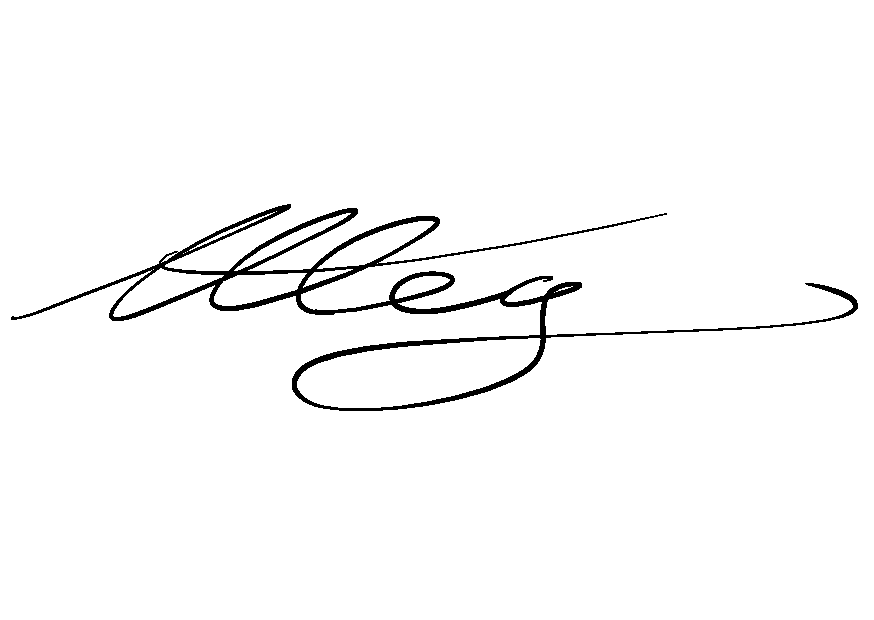
\includegraphics[clip, trim=0cm 3cm 0cm 2cm, width=0.4\textwidth]{../../../signature.pdf}

April Herwig
\newpage

\section*{Abstract}

Koopman operator theory converts traditional analysis of nonlinear dynamical systems into 
analysis of composition operators, allowing one to use mature tools from linear functional 
analysis but requires working in infinite dimensional space. Common Petrov-Galerkin 
methods for Koopman operator analysis suffer from \emph{spectral pollution} - elements 
in the approximated spectrum which are caused solely by discretization and do not 
approximate elements in the true spectrum of the Koopman operator. Resolvent-based 
algorithms to identify spectral pollution are studied, resulting in new connections and 
insights about existing methods, as well as a new method based on previous work. 
Moreover, the notion of "true" Koopman spectrum is critically investigated. 
